
\section{Fejleszt\H oi dokument\'aci\'o}


\subsection{A feladat r\'eszletes le\'ir\'asa}
\subsubsection{Modell}
Adott egy hangull\'am, ami a leveg\H o nyom\'asa az id\H o f\"uggv\'eny\'eben:
\(s: \mathbb{T} \rightarrow \mathbb{P} \) \newline
A modell\"unkben $\mathbb{T}:=[0,+\infty), \mathbb{P}:=[-1,1] $ \newline
A hanghull\'am, mint \"osszetett rezg\'es fel\'irhat\'o k\"ul\"onb\"oz\H o amplit\'ud\'oj\'u, f\'azis\'u \'es frekvenci\'aj\'u harmonikus rezg\'esek (r\'eszhangok) \"osszegek\'ent, azaz: \newline
\( s(t) = \sum_i r_i\cdot\sin{(f_i\cdot t + \varphi_i)} \), ahol $r_i$ az amplit\'ud\'oja, $f_i$ a frekvenci\'aja, $\varphi_i$ pedig a f\'azisa az $i$-edik r\'eszhangnak.
\subsubsection{Specifik\'aci\'o}
\paragraph{Bemenet}
A modellben szerepl\H o $s$ f\"uggv\'enyb\H ol $\Delta t$ id\H o alatt egy $N$ elem\H u mint\'at v\'etelez\"unk: $s_1,\dots,s_{N}$, \'es \newline
\( \begin{array}{rcl}
s_i := s(x_i) & \text{, ahol } & i\in[1..N],\\
&&x_i\in\{ t_0 = x_0 < x_1 < \dots < x_{N-1} = t_0 + \Delta t \} \text{, tov\'abb\'a } \\
&&x_j - x_{j-1} = \frac{\Delta t}{N}\ (j\in[2..N] ) 
\end{array} \)
\paragraph{Kimenet}
Legyen $\mathbb{F}:=\left[ 0..\frac{N}{2} \right]$\newline>
Ekkor a kimenet egy olyan $R_{s,t_0}:\mathbb{F} \rightarrow [0,+\infty)$ f\"uggv\'eny, amely a frekvencia f\"uggv\'eny\'eben megadja az $s\rvert_{[t_0,t_0+\Delta t]}$ hanghull\'amban az adott frekvenci\'aj\'u r\'eszhang amplit\'ud\'oj\'at, azaz $R_{s,t_0}(f_i) = r_i$.
\paragraph{\'Abr\'azol\'as}
Maga a spektrogram az al\'abbi f\"uggv\'ennyel \'irhat\'o le:
\[ \begin{aligned}[rl]
S&:\mathbb{T}\times\mathbb{F} \rightarrow [0,+\infty), \\
S&(t,f):=R_{s,t}(f)
\end{aligned}
\]
Ekkor az \'abr\'azol\'as az $S$ f\"uggv\'eny grafikonj\'anak, azaz
\[
\graf S = \left\{ \big( (t,f) ,S(t,f) \big) : t\in [0,+\infty), f\in\mathbb{F} \right\}
\]




\subsection{Implement\'aci\'o}

\subsubsection{Architekt\'ura}
Az alkalmaz\'as k\'etr\'eteg\H u modell-n\'ezet architekt\'ura szerint k\'esz\"ult.
Ezek m\H uk\"od\'es\'et a \code{VisaulizationApplication} oszt\'aly k\"oti \"ossze \'es ir\'any\'itja.

\paragraph{Alkalmaz\'as}
\begin{figure}[h]
	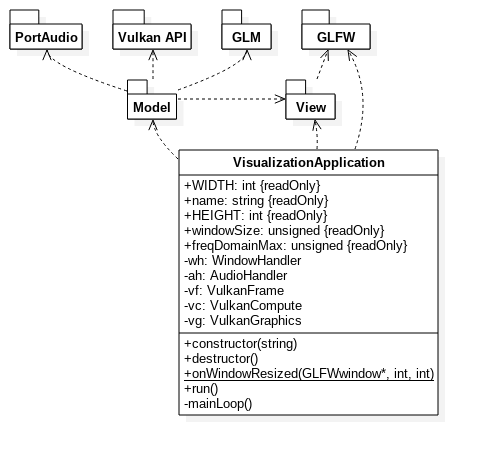
\includegraphics[width=\textwidth]{VisualizationApplication__VisualizationApp_0}
	\centering
	\caption{Az alkalmaz\'as oszt\'alydiagramja \'es a csomagkapcsolatok}
\end{figure}

Az alkalmaz\'as nev\'et a konstruktorban lehet be\'all\'itani, majd a \code{run} met\'odussal elind\'itani. \'Igy a \code{src/main.cpp} f\'ajlban tal\'alhat\'o \code{main} f\"uggv\'enynek csak az alkalmaz\'as futtat\'asa \'es a program sor\'an eldobott kiv\'etelek legv\'egs\H o elkap\'asa lesz a feladata.
Maga az alkalmaz\'as a k\"ovetkez\H o v\'altoz\'okon kereszt\"ul param\'eterezhet\H o:
\begin{itemize}
	\item \code{WIDTH} \'es \code{HEIGHT}: a megjelen\'it\H o ablak kezdeti m\'erete.
	\item \code{windowSize}: mekkora legyen a minta, amit elemz\"unk; a specifik\'aci\'oban $N$
\end{itemize}

\paragraph{N\'ezet}
\begin{figure}[h]
	\includegraphics[width=\textwidth]{View__ViewClassDiagram_2}
	\centering
	\caption{A n\'ezet r\'eteg}
\end{figure}
Az alkalmaz\'as fel\"ulete egy darab megjelen\'it\H o ablakb\'ol \'all, ez a prezent\'aci\'os fel\"ulet.
Ezt a \code{WindowHandler} oszt\'aly biztos\'itja, a GLFW k\"onyvt\'ar seg\'its\'eg\'evel. \newline
A konstruktor\'aban inicializ\'alja a GLFW-t, l\'etrehozza \'es be\'all\'itja az ablakot, be\'all\'itja a hibakezel\H o f\"uggv\'eny\'et. \newline
A \code{getGLFWextensions} f\"uggv\'ennyel inform\'aci\'ot szerezhet\"unk a k\"onyvt\'art\'ol, hogy milyen kieg\'esz\'it\H o funkcionalit\'asokra lesz sz\"uks\'eg\"unk a z\"okken\H omentes m\H uk\"od\'eshez. Ezt felhaszn\'aljuk amikor egy kompatibilis fizikai eszk\"ozt keres\"unk.

\paragraph{Modell}
A modell r\'eteg tov\'abbi r\'eszekre bonthat\'o.
\begin{figure}[h]
	\includegraphics{}
\end{figure}

\subparagraph{Hangkezel\'es}
A hang kezel\'es\'et az \code{AudioHandler} oszt\'aly biztos\'itja.
TODO: interf\'essz\'e alak\'it\'as, \'es k\"ul\"on TestAudioHandler illetve MicAudioHandler.

\subparagraph{Hangfeldolgoz\'as}
A hangfeldolgoz\'as a specifik\'aci\'oban eml\'itett m\'odon diszkr\'et Fourier-transzform\'aci\'oval t\"ort\'enik, ami a \code{VulkanCompute} oszt\'aly seg\'its\'eg\'evel vide\'ok\'arty\'an t\"ort\'enik.
A konstruktor\'aban l\'etrehozza a m\H uk\"od\'es\'ehez sz\"uks\'eges eszk\"oz\"oket. 
\begin{itemize}
	\item A logikai eszk\"ozt, amin kereszt\"ul a program a fizikai eszk\"ozzel kommunik\'alni tud.
	\item A logikai eszk\"ozh\"oz tartoz\'o sort, ahova az utas\'it\'asokat lehet k\"uldeni.
	\item Mem\'ori\'at allok\'al az eszk\"ozon.
	\item Buffereket hoz l\'etre a mem\'oria el\'er\'es\'ere.
	\item L\'etrehozza az er\H oforr\'as le\'ir\'okat.
	\item Bet\"olti a sz\'am\'it\'ast defini\'al\'o shadert.
	\item Sz\'am\'it\'asi cs\H ovezet\'eket hoz l\'etre.
	\item Command pool-t kre\'al \'es command buffer-t foglal bel\H ole.
	\item Felveszi a majd v\'egrehajtand\'o parancsokat a command buffer-be.
\end{itemize}

Ezek ut\'an haszn\'alatra k\'esz, amely sorrendje:
\begin{enumerate}
	\item Adatok felt\"olt\'ese a mem\'ori\'aba a \code{copyDataToGPU} f\"uggv\'eny seg\'its\'eg\'evel.
	\item A sz\'am\'it\'as futtat\'asa a \code{runCommandBuffer} met\'odus megh\'iv\'asa \'altal.
	\item A sz\'amolt eredm\'eny kiolvas\'as\'a a \code{readDataFromGPU} f\"uggv\'ennyel.
\end{enumerate}
TODO: A sz\'amol\'o \'es a rajzol\'o haszn\'aljon k\"oz\"os mem\'ori\'at.

\subparagraph{Rajzol\'as}

%these two may be the same
%\input{tex/dev/application}

\subsection{El\H ok\"ovetelm\'enyek}
\subsubsection{Vide\'ok\'artya driver}
A haszn\'alt Linux disztrib\'uci\'o csomagjai k\"oz\"ott \'erdemes a \code{vulkan} kulcssz\'ora r\'akeresni \'es a haszn\'alt hardvernek megfelel\"o csomagot/csomagokat feltelep\'iteni.
\subsection{K\"onyvt\'arak}

\subsubsection{Audio}

\subsubsection{Vulkan SDK}
\paragraph{Bevezet\H o}
A LunarG Vulkan SDK sz\'amos elengedhetetlen eszk\"ozt tartalmaz. K\"ozt"uk a sz\"uks\'eges fejl\'eceket, a standard valid\'aci\'os r\'etegeket, debuggol\'o eszk\"oz\"oket \'es a Vulkan f\"uggv\'enyek bet\"olt\H oj\'et. 
\paragraph{Telep\'it\'es}
A haszn\'alt Linux disztrib\'uci\'o csomagjai k\"oz\"ott val\'osz\'in\"uleg megtal\'alhat\'oak fejleszt\'eshez sz\"uks\'eges csomagok. 
\newline
Ellenkez\H o esetben a weboldalr\'ol (\url{https://vulkan.lunarg.com/sdk/home}) let\"olthet\H o a legfrissebb SDK verzi\'o.
A script futtat\'asa ut\'an lesz egy \code{VulkanSDK} mappa az adott k\"onyvt\'arban.
Az ebben tal\'alhat\'o \code{Getting\_Started.html} f\'ajl j\'o kiindul\'opont a tov\'abbiakhoz.
A \code{setup-env.sh} script automatikusan be\'all\'itja a sz\"uks\'eges k\"ornyezeti v\'altoz\'okat.
\paragraph{Tesztel\'es}
Ezek ut\'an a \code{vulkaninfo}\footnote{A \code{vulkaninfo --html} paranccsal egy k\"onnyeben b\"ong\'eszhet\H o weboldalt kapunk kimenetnek.} parancsot kiadva inform\'aci\'okat kaphatunk a rendszer\"unk k\'epess\'egeir\H ol, illetve tesztelhetj\"uk az SDK telep\'it\'es\'enek sikeress\'eg\'et. 
\'Erdemes lehet tov\'abb\'a p\'eldaprogramokat is lefuttatni. A \code{build\_examples.sh} script leford\'itja a p\'eldaprogramokat, amik ut\'ana a \code{examples/build/} k\"onyvt\'arban megtal\'alhat\'oak. (\code{cube, cubepp})

\subsubsection{GLFW}
A megjelen\'it\H o ablak kezel\'es\'ere a GLFW k\"onyvt\'arat haszn\'alom. Ez szint\'en telep\'ithet\H o csomag a legt\"obb Linux disztrib\'uci\'oban, vagy a weboldalukr\'ol let\"olthet\H o \'es telep\'it\'esi \'utmutat\'as is megtal\'alhat\'o. \url{http://www.glfw.org/download.html}

\subsubsection{GLM}
Az OpenGL-b\H ol ismer\H os matematikai k\"onyvt\'ar. 
A telep\'it\'ese t\"ort\'enhet csomagkezel\H on kereszt\"ul, vagy mivel csak fejl\'eceket tartalmaz\'o k\"onyvt\'ar, a megfelel\H o helyre let\"olt\'essel.

\subsection{Ford\'it\'as}
A program gy\"ok\'erk\"onyvt\'ar\'aban vagyunk
a \code{make} parancs kiad\'as\'aval a k\"ovetkez\H ok t\"ort\'ennek:
\begin{enumerate}
	\item Leford\'itjuk a shadereket (ld. \ref{shadercompilation})
	\item Leford\'itjuk a programot (ld. \ref{compileoptions})
\end{enumerate}

\subsubsection{Ford\'it\'o v\'alaszt\'asa}
A \code{Makefile} elej\'en a \code{COMPILER} v\'altoz\'ot a k\'iv\'ant ford\'it\'ora kell \'all\'itani (\code{g++/clang++}).
\subsubsection{Ford\'it\'asi param\'eterek}\label{compileoptions}
A teljes parancs (a \code{Makefile}-b\'ol): 
\begin{itemize}
	\item Debug verzi\'o
		%\code{\$(COMPILER) -o \$(DTARGET)/\$(OUTPUT_NAME) \$(SOURCES) \$(CFLAGS) \$(INCLUDE) \$(LDFLAGS) -DDEBUG -g -ggdb}
	\item Release verzi\'o
		%\code{\$(COMPILER) -o \$(TARGET)/\$(OUTPUT_NAME) \$(SOURCES) \$(CFLAGS) \$(INCLUDE) \$(LDFLAGS) -DNDEBUG }
\end{itemize}
Itt a k\"ulonb\"oz\H o v\'altoz\'ok:
\begin{itemize}
	\item \code{COMPILER}: A v\'alasztott ford\'it\'o (\code{gcc} vagy \code{clang})
	\item \code{TARGET/DTARGET}: A c\'elmappa (\code{bin/debug} vagy \code{bin/release}) 
	\item \code{OUTPUT\_NAME}: A futtathat\'o \'allom\'any neve
	\item \code{SOURCES}: Az \code{src} k\"onyvt\
	\item \code{CFLAGS}: 
	\item \code{INCLUDE}: 
	\item \code{LDFLAGS}: 
\end{itemize}

\subsubsection{Shader}\label{shadercompilation}
A Vulkan API SPIR-V (\url{https://www.khronos.org/spir/}) shadereket haszn\'al. Mivel ez egy b\'ajtk\'od form\'atum, \'igy a shaderek manu\'alis \'ir\'asa \'es olvas\'asa szokatlan lehet. 
Szerencs\'ere a Khronos Group lefejlesztett egy ford\'it\'ot, ami az OpenGL-b\H ol ismer\H os GLSL shadert SPIR-V shaderr\'e alak\'itja. A LunarG SDK-ban megtal\'alhat\'o ez a program, a 
\code{glslangValidator}. \newline
A GLSL shaderek ford\'it\'asa \'igy t\"obbf\'elek\'eppen is t\"ort\'enhet:
\begin{itemize}
	\item \code{make shaders} \newline
		A \code{Makefile}-ban defini\'alt parancs, leford\'tja az \"osszes shadert a \code{src/shaders} mapp\'aban.
	\item \code{glslangValidator -V src/shaders/<shader neve>} \newline
		A \code{-V} kapcsol\'o mondja meg, hogy gener\'aljon is SPIR-V shadert, an\'elk\"ul csak ellen\H orzi a k\'odot, hogy megfelel-e az implement\'alt szabv\'anynak.
\end{itemize}



\subsection{Tesztel\'es}
